\graphicspath{{Ch4_Jets/figures/}}

\chapter{Jets}
%TODO: reference boson tagging part of analysis chapter somewhere in this chapter
%TODO: basic jet cartoon figure
%TODO: discuss boosted hadronic decays and two-pronged structure relevant to this analysis
As discussed in Section~\ref{sec:monte_carlo}, partons created during $pp$ collisions undergo a showering process where they produce cascades of additional strongly interacting particles through gluon radiation and splitting.
As this showering process concludes and the products approach a sufficiently low energy ($\approx 1$ GeV) the resulting partons hadronize and produce a spray of colorless hadrons called a ``jet'' which interacts with both the tracking and calorimeter systems of the ATLAS detector.
Jets are reconstructed by employing \textit{jet clustering algorithms} which take a set of constituent inputs from the event and combine them to output a set of jets.
At the ATLAS experiment jets may be constructed using only tracks as inputs, only calorimeter clusters and inputs, or a combination of both.

\section{Jet Constituents}
\label{sec:jet_constituents}
All jet clustering algorithms take as input a set of four-vectors representing all the products of parton showering and hadronization, known as \textit{constituents}.
These constituents compose \textit{all} the potential jets in the event, and it is the job of the jet clustering algorithm to convert these to a set of four-vectors representing only the corresponding jets from the event.
These constituents can be created with information from any particular ATLAS sub-detector or combination thereof, as long as they encode the four-vectors of the particles produced during the jet showering/hadronization process.
The most relevant constituent types for this analysis are outlined below.

\subsection{Calorimeter Clusters}
The information quality contained within a collection of calorimeter signals of a given collision event can be increased by grouping the signals into \textit{topologically connected cell clusters}.
This strategy helps to reduce the impact of background electronic noise and other sources of calorimeter fluctuation such as the presence of pile-up.
The finely segmented lateral ($\eta$-$\phi$) readout together with the longitudinal sampling layers allows the ATLAS calorimeter system to resolve spatial signal patterns relevant for jet reconstruction while efficiently removing insignificant signals caused by noise.

\newcommand{\LCTopoSig}{\ensuremath{\varsigma^{\mathrm{EM}}_{\mathrm{cell}}}}
These topo-clusters are formed by a growing-volume algorithm \cite{Aad:2016upy} which begins with a calorimeter cell possessing a highly significant \textit{seed signal}, where significance is defined as the ratio of the cell signal magnitude over the expected noise:
\begin{equation}
    \LCTopoSig = \frac{E^{\mathrm{EM}}_{\mathrm{cell}}}{\sigma^{\mathrm{EM}}_{\mathrm{noise,cell}}}
    \label{eqn:lctopo_sig}
\end{equation}
The growth of the topo-cluster proceeds iteratively by connecting nearby cells, where the seeding, growth, and boundary conditions are controlled by placing bounds on the cell significance (Eq.~\ref{eqn:lctopo_sig}), as shown in Figure~\ref{fig:lctopo_formation}.
The four-vector corresponding to each topo-cluster is computed by a weighted combination of all cells contained in the topo-cluster.
The weights are necessary because each cell is allowed to contribute (unevenly) its energy to two separate topo-clusters.

\begin{figure}
	\centering
	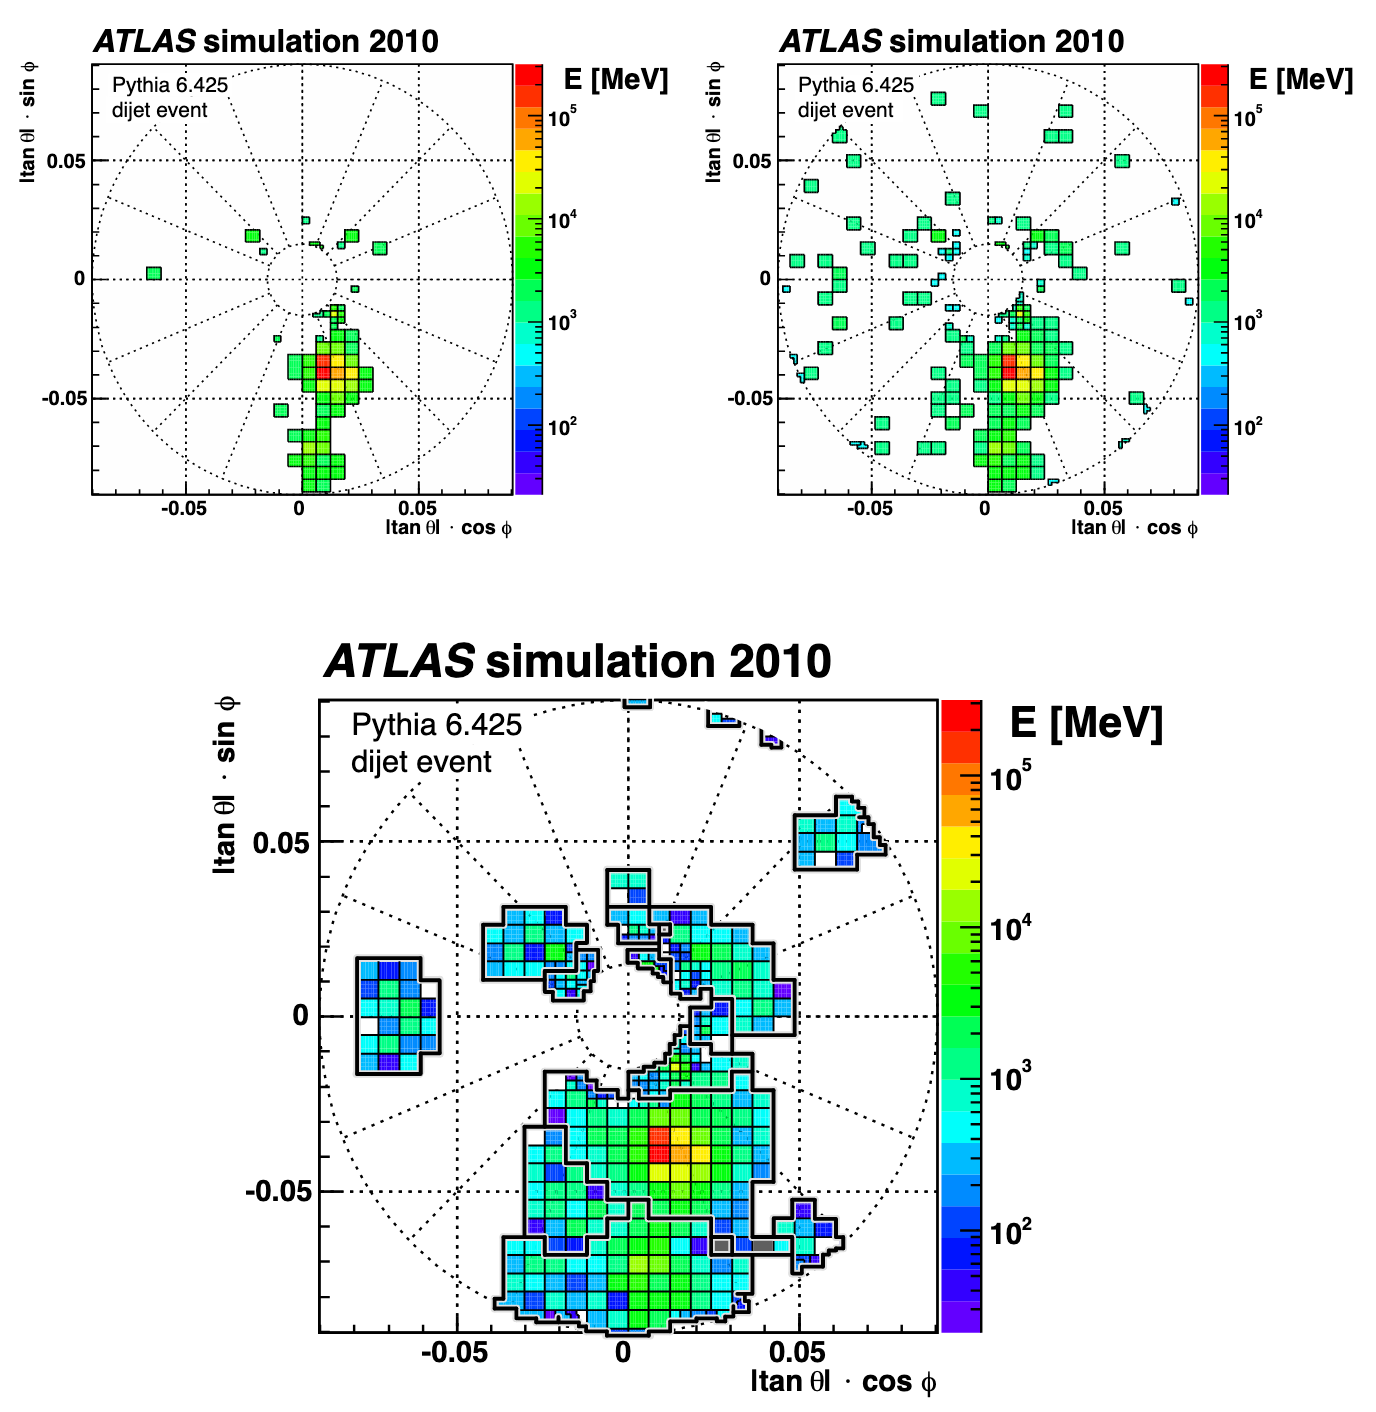
\includegraphics[width=\textwidth]{lctopo_formation}
	\caption{
	Stages of topo-cluster formation in the FCAL calorimeter for a simulated dijet event.
	Cells with $\LCTopoSig > 4$ (top left) are used in the seeding, cells with $\LCTopoSig > 2$ (top right) control the topo-cluster growth.
	The final set of topo-clusters (bottom) is shown with black outlines around each cluster.
	Adapted from \cite{Aad:2016upy}.
	}
	\label{fig:lctopo_formation}
\end{figure}

\subsection{Tracks}
The more energetic or ``boosted'' a jet-initiating particle is, the more collimated the showering/hadronization process becomes.
At a certain point the calorimeter resolution is no longer fine-grained enough to fully resolve the individual jet constituents.
On the other hand, the ID has excellent angular resolution and track reconstruction efficiency even at very high energy with dense clusters of charged particles \cite{Aaboud:2017all}.
Since jet clustering algorithms are indifferent to the origin of the inputs, only requiring a set of four-vectors as input, they can be applied to tracks just as well as calorimeter clusters.
In particular, utilizing ID information during jet clustering allows for a more detailed view of the internal structure of jets, which is particularly useful in the context of jet substructure (Section \ref{sec:jet_substructure}) and $b$-tagging (Section \ref{sec:btagging}).

\subsection{Track-Calo Clusters}
\label{sec:tcc_constituents}
% cite combined mass as first step towards TCCs
\newcommand{\mCALO}{\ensuremath{m^{\mathrm{calo}}}}
\newcommand{\mTRACK}{\ensuremath{m^{\mathrm{track}}}}
\newcommand{\mTA}{\ensuremath{m^{\mathrm{TA}}}}
\newcommand{\ptCALO}{\ensuremath{p_T^{\mathrm{calo}}}}
\newcommand{\ptTRACK}{\ensuremath{p_T^{\mathrm{track}}}}
While using tracks as inputs to the jet clustering improves the angular resolution, there are two primary downsides: (1) only charged particles interact with the ID, and (2) the energy resolution of the tracking detector degrades at very high energy.
In order to achieve the best of both worlds, tracking and calorimeter information can be combined.
One of the first ways in which ATLAS explored this possibility was by improving the calorimeter jet mass $(\mCALO)$ measurement by incorporating information about nearby associated tracks to produce the so-called \textit{track-assisted jet mass} \cite{ATLAS-CONF-2016-035}.

The four-vector of a jet is simply the sum of the four-vectors of its constituents. For a calorimeter jet $J$ with calorimeter cell cluster constituents $i$, each with momentum $\vec{p}_i$, the calorimeter mass ($\mCALO$) is defined (by the basic rules of special relativity) as:
\begin{equation}
    \mCALO = \sqrt{
        \left(
            \sum_{i \in J} E_i
        \right)^2
            -
        \left(
            \sum_{i \in J} \vec{p}_i
        \right)^2
    }
    \label{eqn:jet_mass}
\end{equation}
and the track-assisted jet mass is defined as:
\begin{equation}
    \mTA = \frac{\ptCALO}{\ptTRACK} \times \mTRACK
    \label{eqn:ta_jet_mass}
\end{equation}
where \ptCALO\ is the transverse momentum of a calorimeter jet, \ptTRACK\ is the transerve momentum of the four-vector sum of tracks associated to the calorimeter jet and \mTRACK\ is the invariant mass of this four-vector sum.
The improvement in jet mass resolution observed with $\mTA$ is shown in Figure~\ref{fig:ta_vs_comb_mass_res}.

\begin{figure}
	\centering
	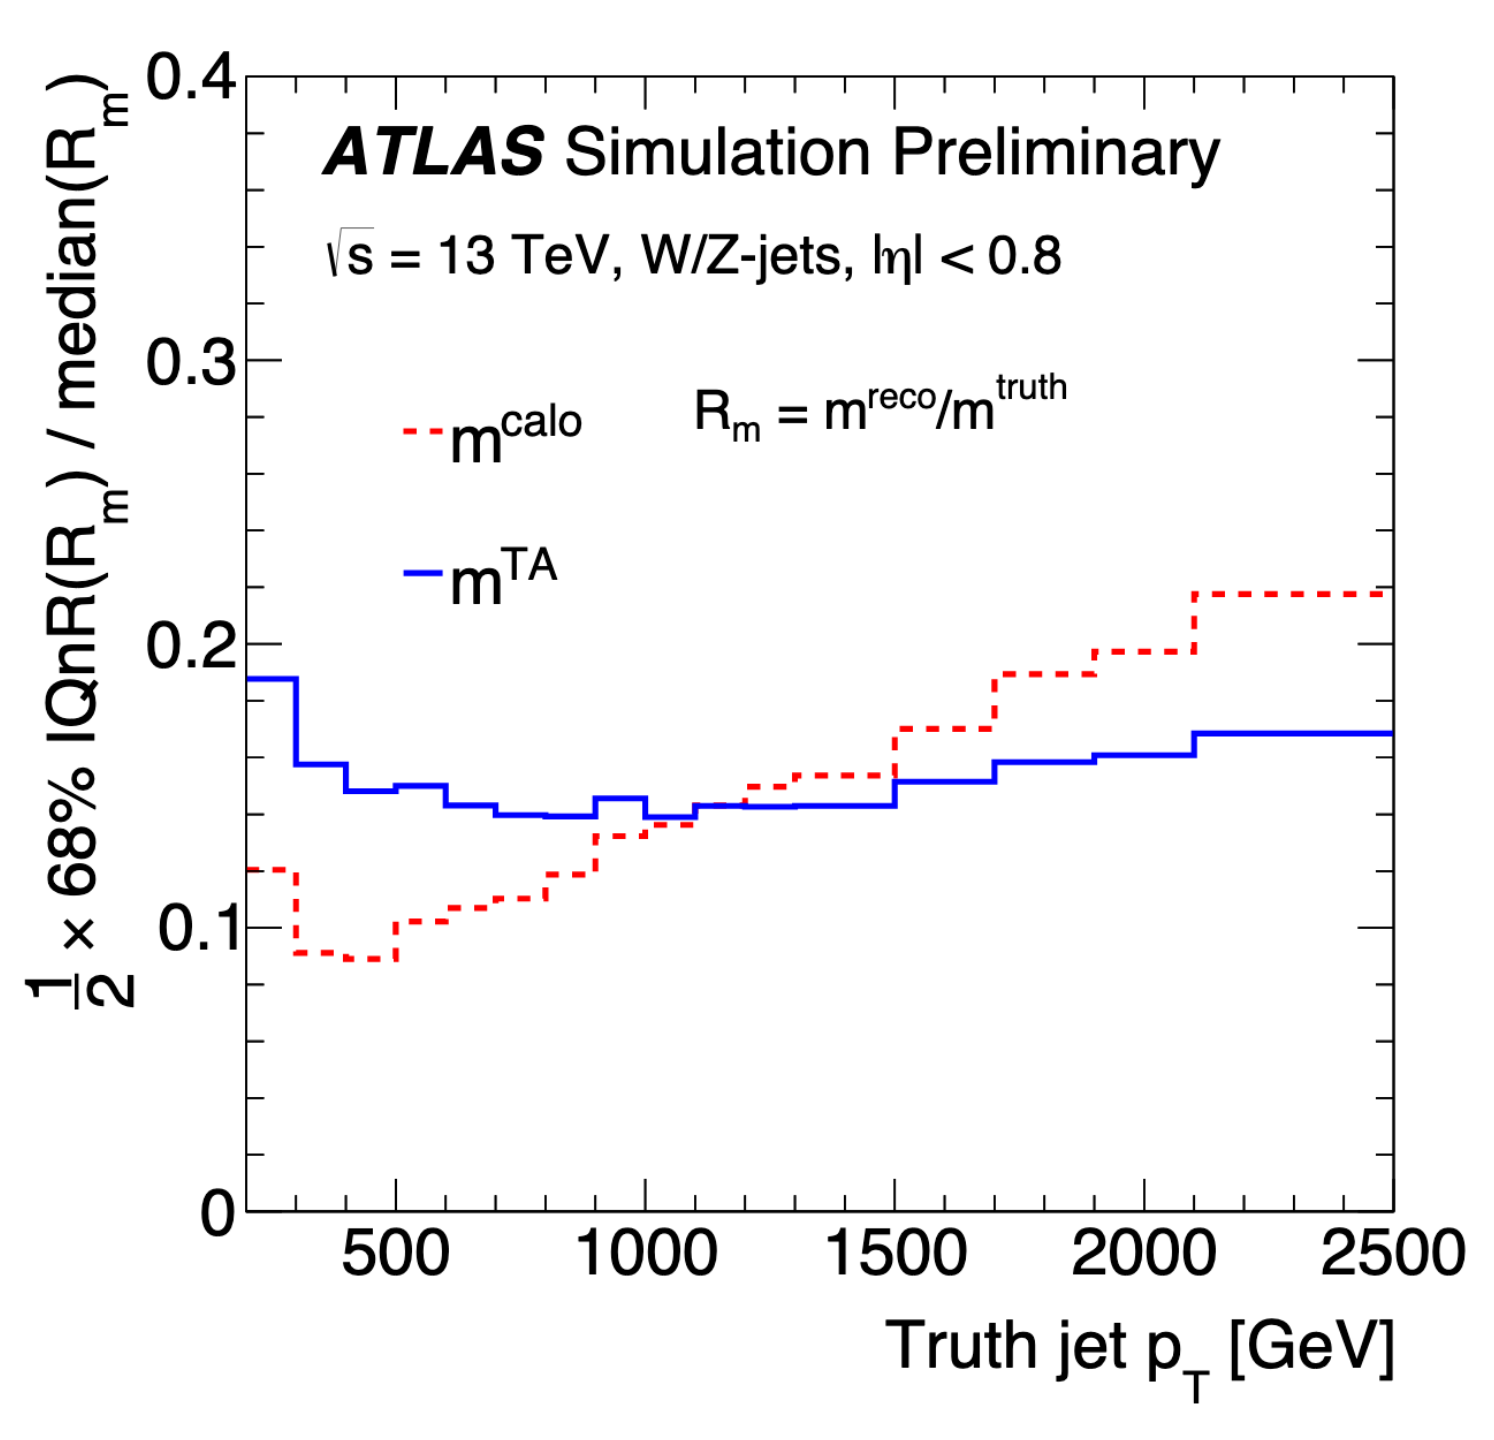
\includegraphics[width=0.6\textwidth]{ta_vs_calo_mass_res_wz_jets}
	\caption{
	The resolution of the jet mass response as a function of truth jet $p_T$ for simulated $W$ and $Z$ boson jets for calorimeter-based jet mass (dashed red line) and track-assisted jet mass (blue solid line).
	The half of the 68\% interquartile range (IQnR) divided by the median of the jet mass response is used as an outlier-insensitive measure of the resolution.
	\cite{ATLAS-CONF-2016-035}
	}
	\label{fig:ta_vs_comb_mass_res}
\end{figure}

While the jet mass resolution is notably improved by utilizing \mTA in many cases, a more rigorous unification of tracking and calorimeter information was desired to yield benefits in \textit{all} observable jet properties at a wider range of energies.
One method to achieve this is the definition of a new type jet input constituent which unifies tracks and calorimeter deposits into new ``Track-Calo Cluster'' (TCC) objects, designed to maximally exploit the strengths of each detector.

To build TCC constituents for each event, good quality tracks matched to the selected hard scatter primary vertex are extrapolated to the calorimeter and matched to corresponding topo-clusters.
The error on this extrapolation accounts for both the original ID measurement of the track parameters, as well as additional uncertainty accumulated as the particle passes through additional detector elements.
The typical extrapolated angular uncertainty of a track is significantly smaller than the size of the average topo-cluster across the detector, particular for moderate to high $p_T$ tracks.

\begin{figure}
	\centering
	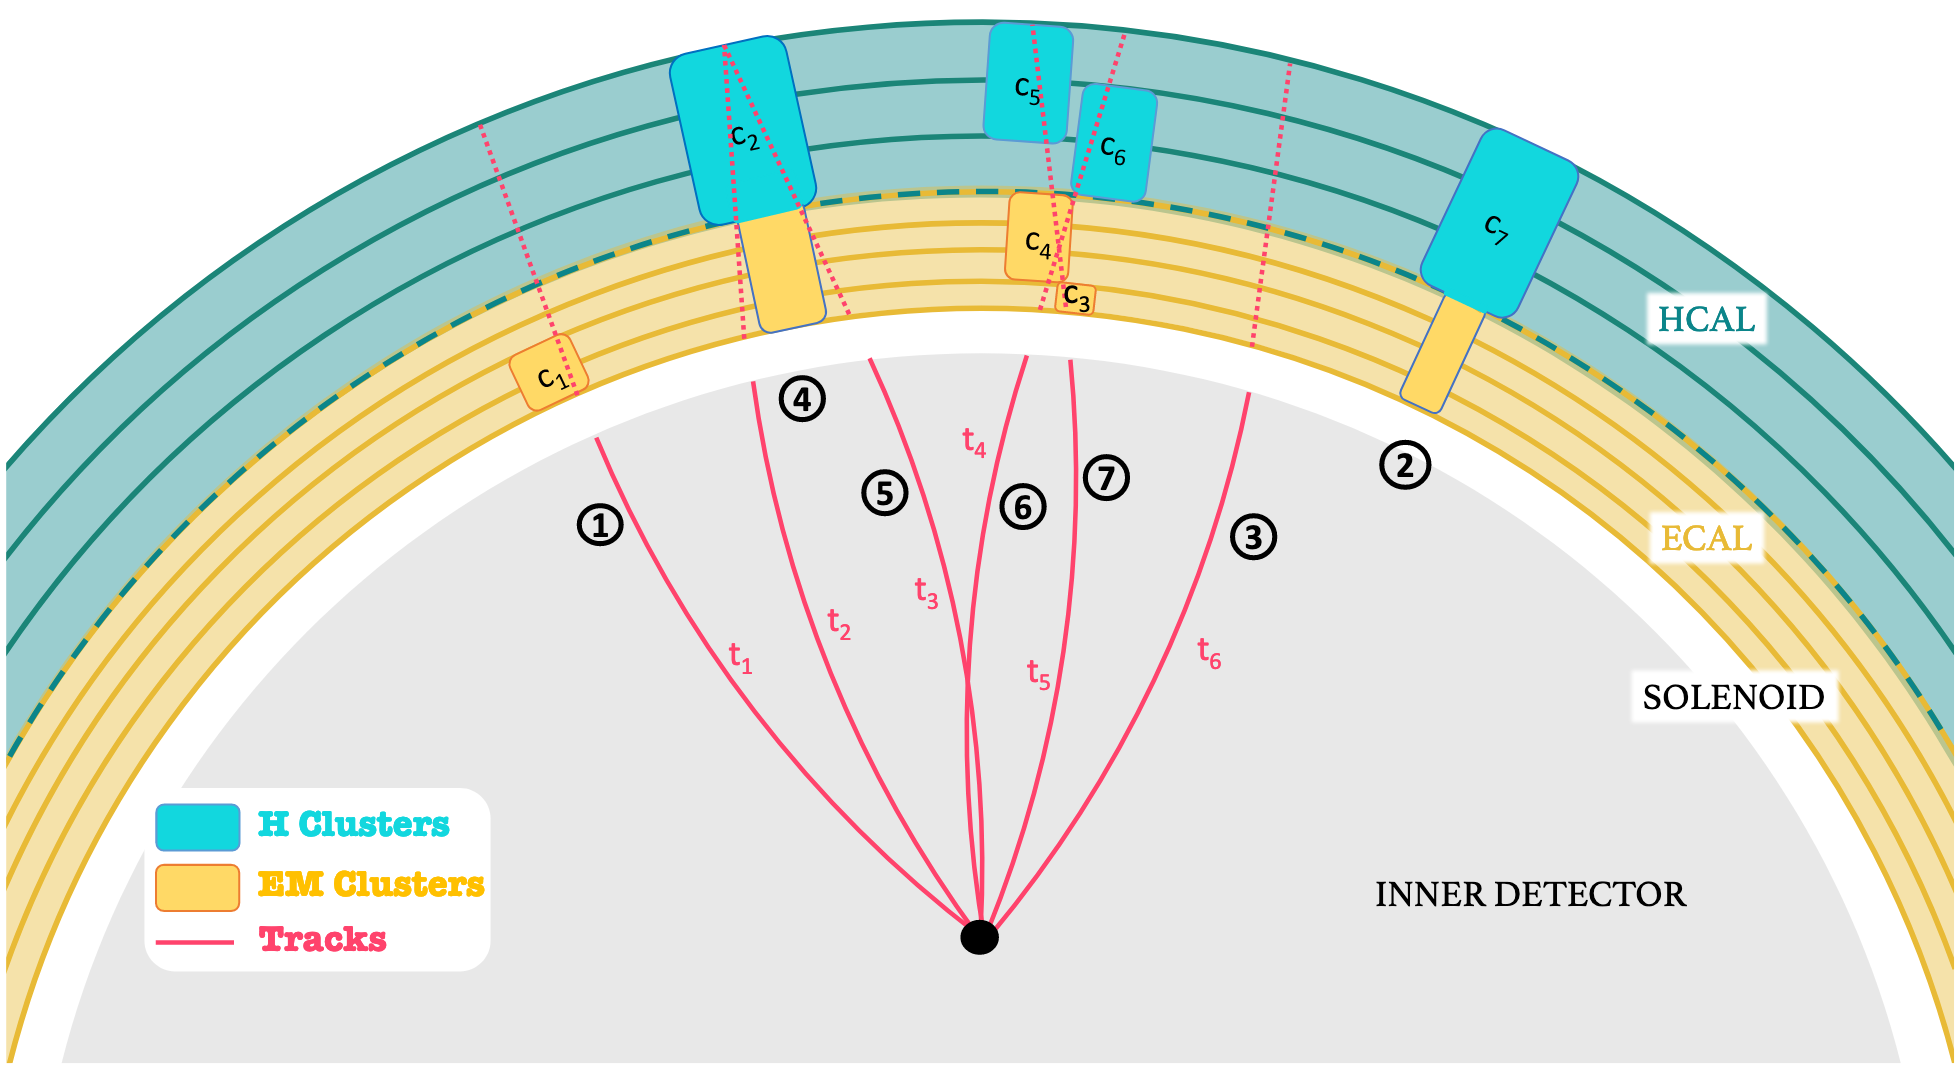
\includegraphics[width=\textwidth]{TCC_cartoon}
	\caption{
	A schematic demonstration the creation of seven TCC objects representing \circled{1} a simple track-cluster match, \circled{2} a topo-cluster without a matching track, \circled{3} a track without a matching cluster, \circled{4} and \circled{5} are each tracks matching a single cluster but sharing that cluster's energy, and \circled{6} and \circled{7} showing a much more complex scenario with multiple track-cluster matches.
    \cite{ATL-PHYS-PUB-2017-015}
	}
	\label{fig:tcc_cartoon}
\end{figure}

Fully matched track/topo-cluster combinations are referred to as ``combined''.
Un-matched topo-clusters and tracks are not discarded, but rather grouped into separate sets of TCC constituents.
TCC objects created with an un-matched track are referred to as ``charged'', and TCC objects created with an un-matched topo-cluster are referred to as ``neutral''.
Within the acceptance of the ID the ``combined'' type composes $> 95\%$ of all reconstructed TCC, whereas outside the acceptance of the ID the ``neutral'' type dominates, as shown in Figure~\ref{fig:tcc_cluster_fractions}.

\begin{figure}
	\centering
	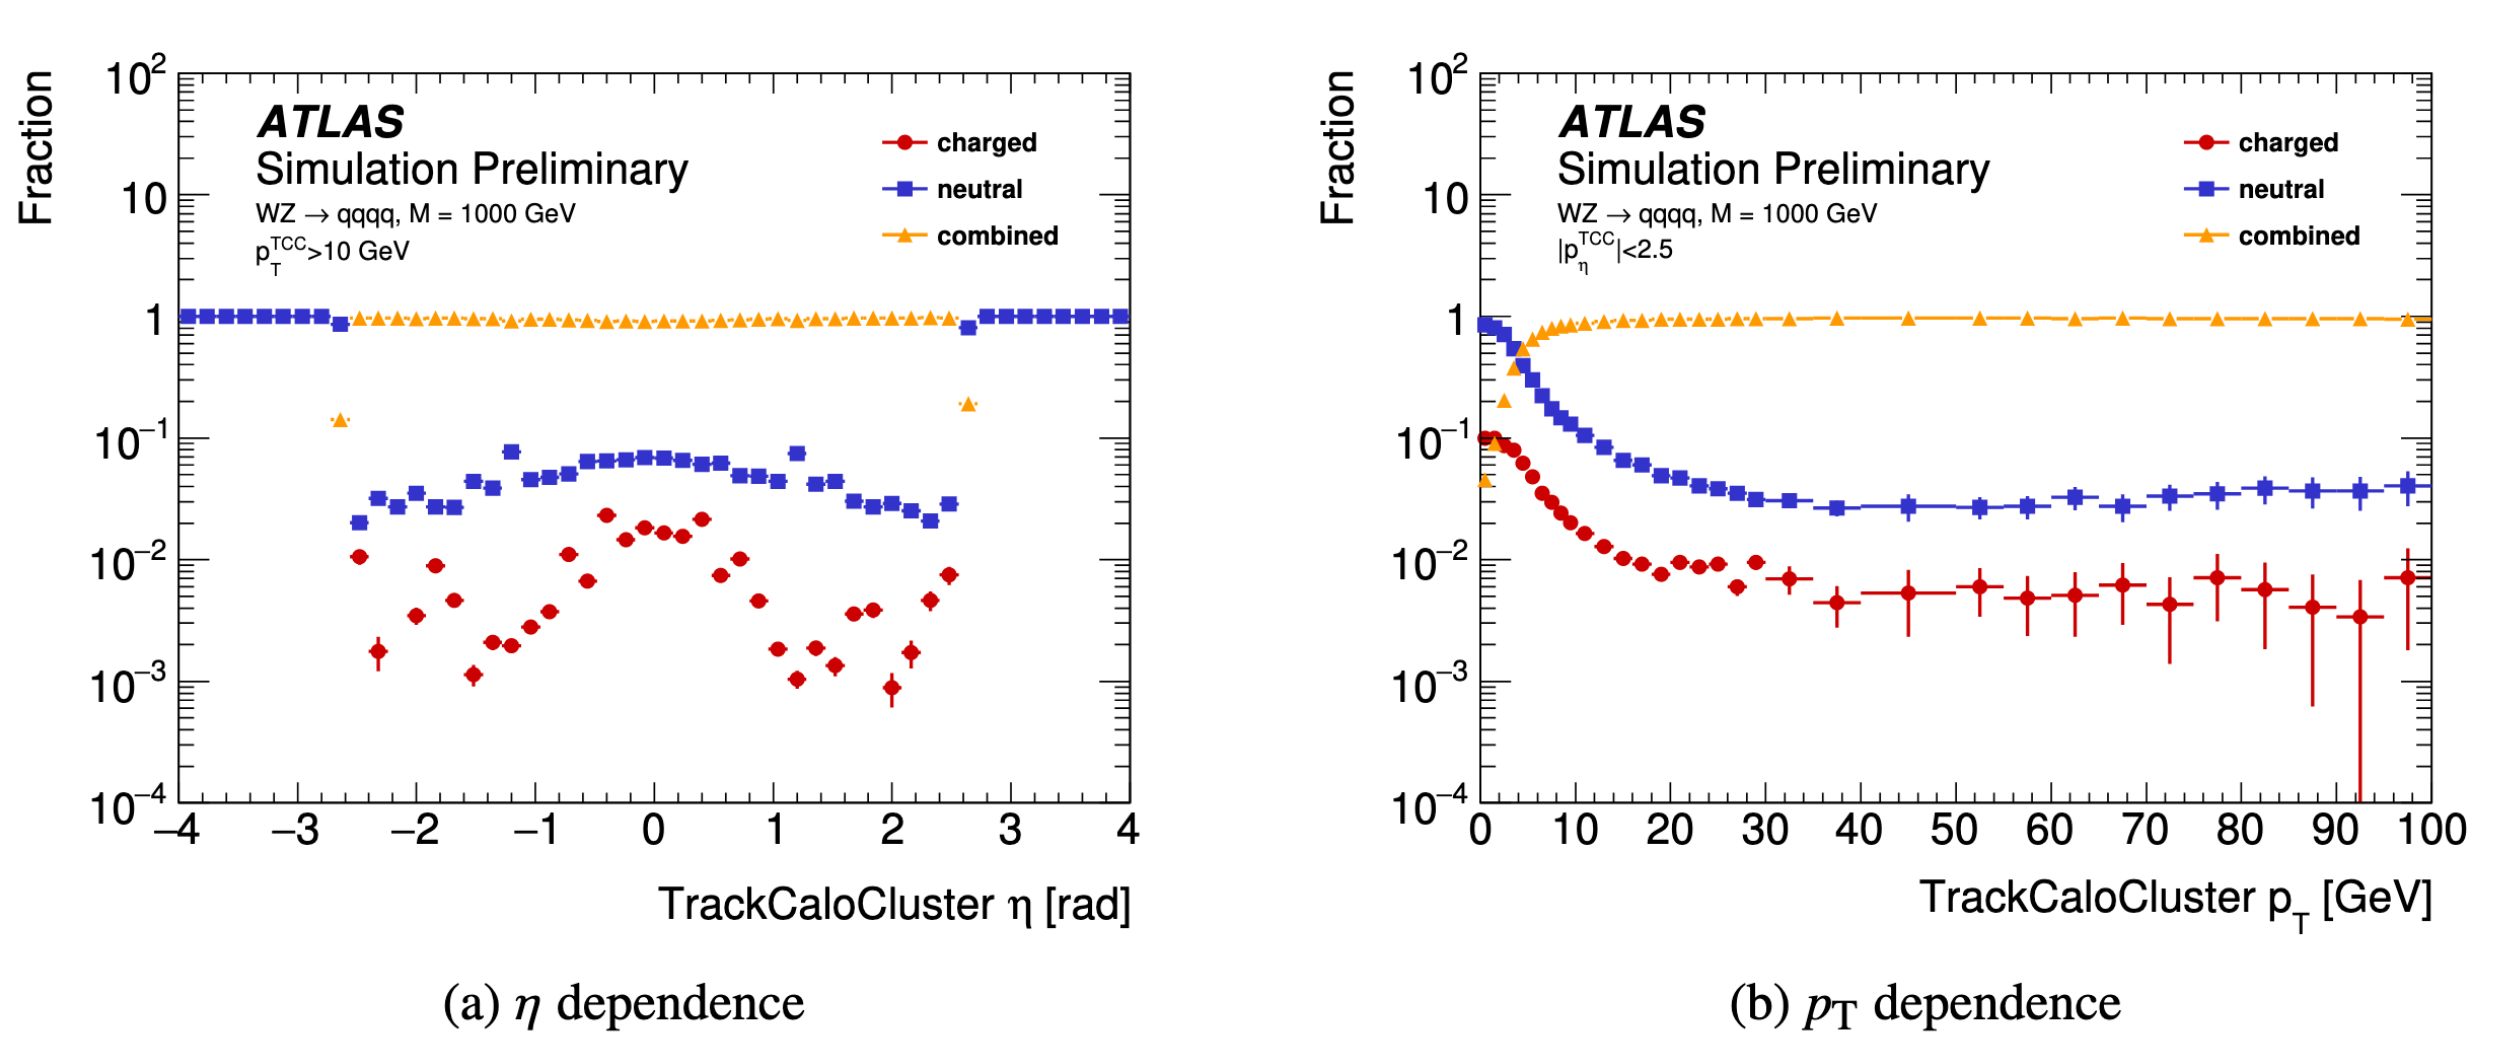
\includegraphics[width=\textwidth]{tcc_cluster_fractions}
	\caption{
	The fractions of different TCC types are shown as a function  of (a) the TCC $\eta$ and (b) the TCC $p_T$.
	Combined objects (triangles) represent tracks for the selected hard scatter primary vertex which are matched to topo-clusters, neutral objects (squares) are for topo-clusters not matched to tracks for any primary vertex, and charged objects (circles) are tracks from the selected hard scatter primary vertex not matched to any topo-cluster.
    \cite{ATL-PHYS-PUB-2017-015}
	}
	\label{fig:tcc_cluster_fractions}
\end{figure}

In order to combine the track and/or topo-cluster into a single object, a scheme must be devised for defining the resulting four-vector in terms of the four-vectors of the track and topo-cluster.
This is done in a straight-forward manner as follows:
\newcommand*\caloP[1]{#1^{\mathrm{calo}}}
\newcommand*\trackP[1]{#1^{\mathrm{track}}}
\begin{align}
    \vec{p}_{\mathrm{TCC}}^{\mathrm{\;combined}} &\equiv (\caloP{p_T}, \trackP{\eta}, \trackP{\phi}, \caloP{m})\\
    \vec{p}_{\mathrm{TCC}}^{\mathrm{\;charged}} &\equiv (\trackP{p_T}, \trackP{\eta}, \trackP{\phi}, \trackP{m})\\
    \vec{p}_{\mathrm{TCC}}^{\mathrm{\;neutral}} &\equiv (\caloP{p_T}, \caloP{\eta}, \caloP{\phi}, \caloP{m})
\end{align}
which combines calorimeter energy/mass measurements and track angular information for the combined TCC objects.
For dealing with cases where multiple tracks are matched to the same topo-cluster (or vice versa) a more complicated formula accounting for energy-sharing is required \cite{ATL-PHYS-PUB-2017-015}. 

\section{Clustering Algorithms}
% TODO: reference other algorithms: CA, kT, mass drop, UFO, particle flow, etc
Due to their aggregate nature, the notion of a \textit{jet} is not as immediately or clearly interpreted as are other physics objects such as electrons, muons, and photons.
This allows for a significant amount freedom in how jets are defined and reconstructed in collider experiments.
Furthermore the manner in which individual constituents are combined, and the characteristic size of the resulting jets (in the $\eta$-$\phi$ plane) can be altered on a per-algorithm basis.
To deal with this ambiguity a set of properties that must be met by any standardized jet definition were outlined in December of 1990 \cite{Huth:217490} as follows:
\begin{enumerate}
    \itemsep0em 
    \item Simple to implement in an experimental analysis.
    \item Simple to implement in a theoretical calculation.
    \item Defined at any order of QCD perturbation theory.
    \item Yield finite cross section at any order of perturbation theory.
    \item Yield a cross section that is \textit{relatively} insensitive to hadronization.
\end{enumerate}
This set of rules allows for better communication between experimental and theoretical physics results, as well as better comparison of results between different collider experiments.

The most common category of jet clustering algorithm used by ATLAS is \textit{sequential recombination} \cite{Catani:1993hr}.
These algorithms are carefully designed to be insensitive to the present of soft (sometimes called ``infrared'') and collinear gluon emission and thus useable in perturbation theory calculations.
These recombination algorithms work iteratively by attempting to work in reverse through the history of the parton shower, starting with the softer final products of the showering/hadronization process recorded by the detector, and working back (ideally) to the original hard collisions product(s) which initiated the jet.

The primary quantities of interest in these algorithms are a distance measure between separate objects $d_{ij}$ and between each object and the ``beam'' $d_{iB}$.
\begin{align}
d_{ij} &= \min\left({p_{T_i}^{2P}, p_{T_j}^{2P}}\right) \times \frac{\Delta R_{ij}^2}{R^2} \\
d_{iB} &= p_{T_i}^{2P}
\end{align}
where $\Delta R_{ij}$ is the angular distance between the $i$-th and $j$-th objects: $\Delta R_{ij}^2 = \Delta \eta_{ij}^2 + \Delta \phi^2$, $p_T$ is the transverse momentum of the object, and the parameters $P$ and $R$ are algorithm parameters which regulate the evolution of the clustering.
Starting with the full set of constituents as objects, the algorithm proceeds by identifying the smallest of all the distance measures $d_{ij}$ or $d_{iB}$.
If the smallest is $d_{ij}$ for some particular $i$/$j$ then it combines the four-vectors of $i$ and $j$ into a new object, otherwise if it is $d_{iB}$ then object $i$ is added to the set of jets to be output at the end of the clustering and discarded from the rest of the calculation.
New distances are calculated accounting for combined objects and the process is repeated until no objects are left, or in other words, all constituents in the event have been recombined into jets.

Different jet clustering algorithms in the sequential recombination family are distinguished by different values for the parameters $P$ and $R$ mentioned above. 
The $k_T$ algorithm \cite{Catani:1993hr} for $P=1$ causes softer (lower $p_T$) particles to be merged first.
This introduces a strong sensitivity to small fluctuations of the energy density in the particle shower.
For this reason it is rarely used in a modern context.
The \textit{Cambridge-Aachen} (C/A) algorithm \cite{Dokshitzer:1997in} for $P=0$ works only with the angular component of the jets by sorting the objects without any reference to $p_T$ in $d_{ij}$.

The \textit{anti}-$k_T$ algorithm \cite{Cacciari:2008gp} for $P = -1$ causes soft particles to cluster together with nearby hard particles before they cluster between themselves. 
This reduces sensitivity to small fluctuations of energy within the parton shower, the primary (undesirable) characteristic of the $k_T$ algorithm.
This property causes a hard particle with no hard neighbors within a distance of $2R$ to accumulate all nearby soft particles within a circle of radius $R$.
This leads to a stability in jet area which is helpful for jet calibration and analysis, which has resulted in anti-$k_T$ being used as the default algorithm for the majority of ATLAS research.

The choice of jet clustering algorithm parameters as well as constituent type depends in part upon the physics analysis goals in question.
In particular circumstances two separate jet algorithms may be used to reconstruct the same event to pick out separate features.
For example, for identifying the decay products of the two-pronged decay of a Standard Model vector boson ($W/Z \rightarrow q\bar{q}^{(\prime)}$), the anti-$k_T$ algorithm with a large radius parameter of $R$ = 1 is used to capture the full jet corresponding to the inclusive $W/Z$ decay.
However, jets with a smaller radius parameter can be used to capture the features of the jets corresponding to the individual quark jets.

In particular for the case of capturing and reconstructing the $b$-quarks from a $H \rightarrow b\bar{b}$ decay, a special modification the jet clustering algorithms discussed above can be made to produce jets with variable radius (VR) \cite{Krohn:2009zg}.
This entails modifying the radius parameter $R$ to depend on jet $p_T$ in the following way:
\begin{equation}
R \rightarrow R_{\mathrm{eff}}(p_T) \equiv \frac{\rho}{p_T}
\end{equation}
where the new constant parameter $\rho$ determines how quickly the effective jet size decreases as the jet $p_T$ increases.
Additionally the VR jet clustering algorithm also imposes a minimum ($R_{\mathrm{min}}$) and maximum ($R_{\mathrm{max}}$) bound on the radius which prevents the jet radii from becoming pathologically small or large.

In practice the VR modification has only been widely used on ATLAS for anti-$k_T$ jets reconstructed with track constituents, in particular for reconstructing the individual $b$-jets from an $H \rightarrow b\bar{b}$ decay process.
The values $\rho = 30$ GeV, $R_{\mathrm{min}} = 0.02$, and $R_{\mathrm{max}} = 0.4$ are used in ATLAS and were derived by scanning each parameter for simulated Higgs jets and maximizing the truth $b$-quark matching efficiency for each subjet as shown in Figure~\ref{fig:vr_jet_optimization}.

\begin{figure}
	\centering
	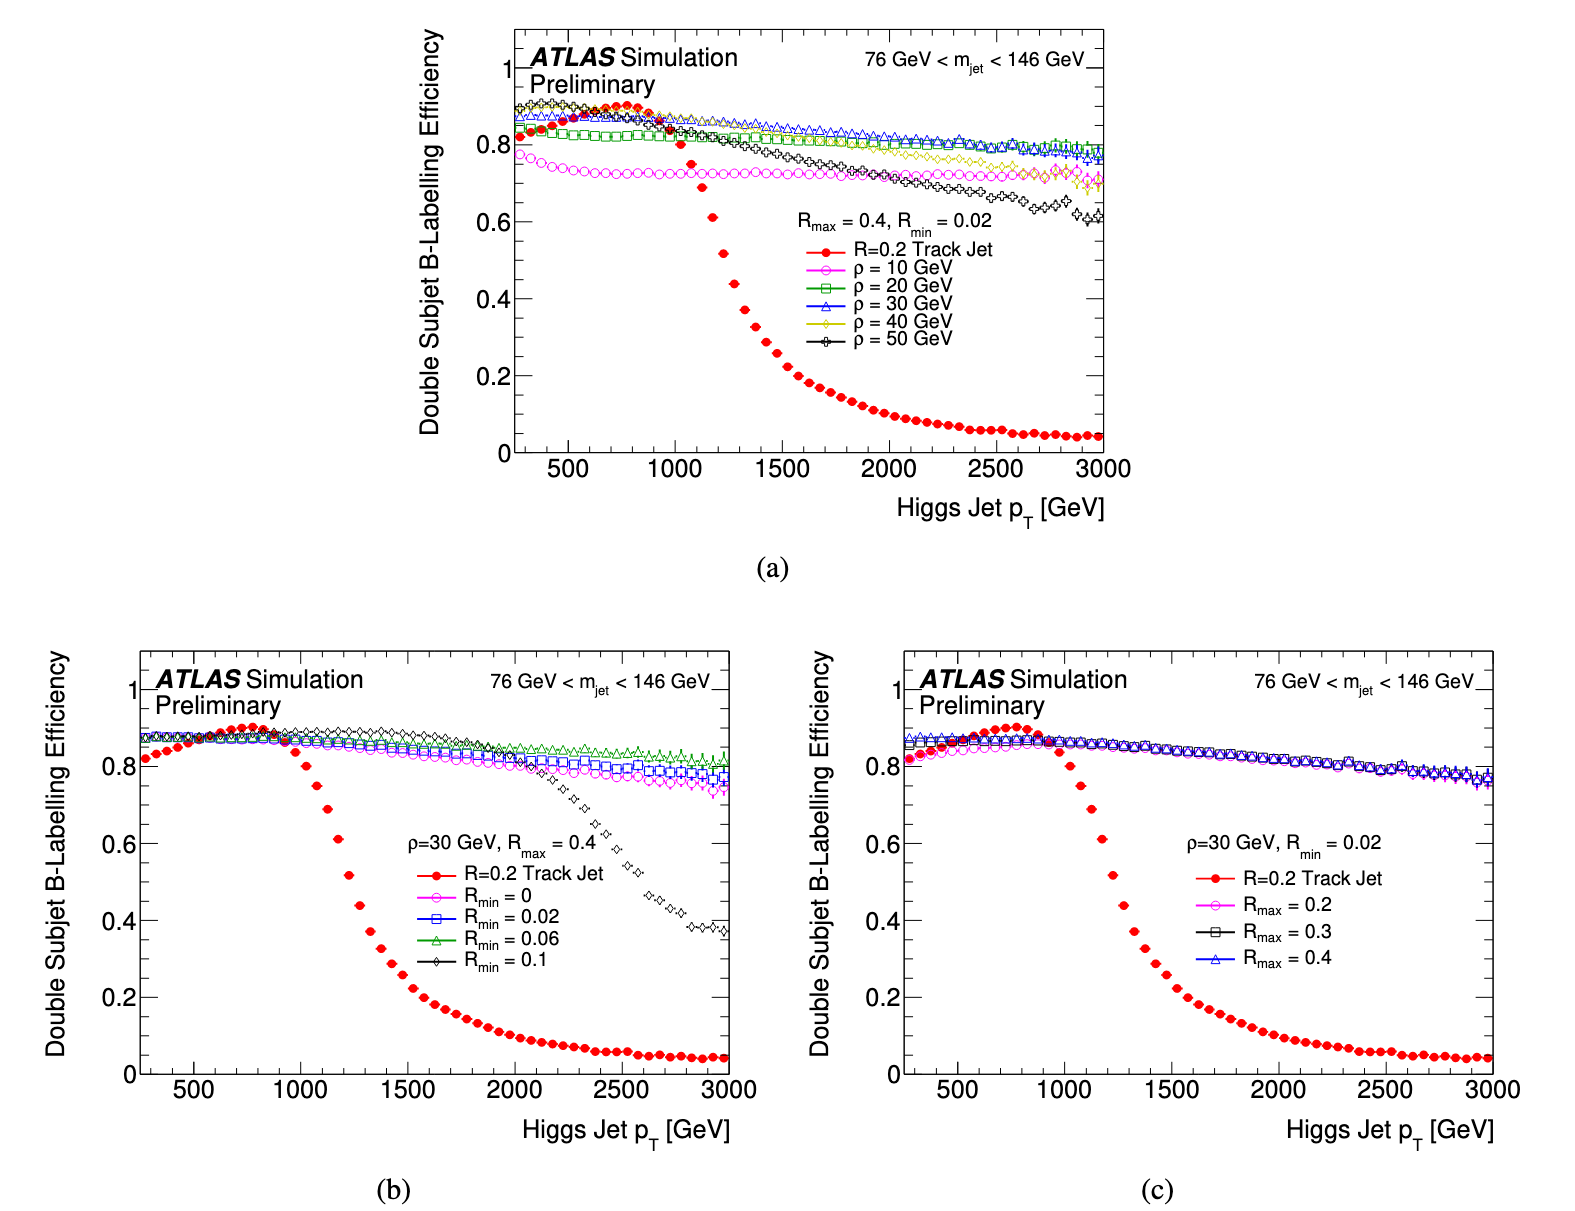
\includegraphics[width=\textwidth]{vr_jet_optimization}
	\caption{
	Efficiency of subjet double $b$-labelling at the truth level for Higgs jets as a function of Higgs jet $p_T$.
	(a) The efficiency for VR track jets with $R_{\mathrm{min}} = 0.02$ and $R_{\mathrm{max}} = 0.4$ for several different $\rho$ values.
	(b) The efficiency for VR track jets with $\rho = 30$ GeV and $R_{\mathrm{max}} = 0.4$ for several different values of $R_{\mathrm{min}}$
	(b) The efficiency for VR track jets with $\rho = 30$ GeV and $R_{\mathrm{min}} = 0.02$ for several different values of $R_{\mathrm{max}}$
	The efficiency for standard $R = 0.2$ track jets is also included in all of the plots.
	}
	\label{fig:vr_jet_optimization}
\end{figure}

\section{Calibration}
\label{sec:jet_calibration}
The jets reconstructed by any particular clustering algorithm may not correctly match the true four-vector of the original parton.
There are a number of factors responsible for this, such as:
\begin{itemize}
    \itemsep0em 
    \item \textbf{Dead Material}: Some of the products of the showering process may be absorbed by inactive detector elements and thus not be present as constituents.
    \item \textbf{Leakage}: Some energy may fall outside or ``punch through'' the calorimeter.
    \item \textbf{Out-of-cone Effects}: Some particles may fall outside the reconstructed jet due to imperfect clustering.
    \item \textbf{Thresholds/Efficiency}: A proportion of the total jet energy may be lost in reconstruction. For example by falling below the noise threshold in some calorimeter cells.
\end{itemize}

In order to compensate for these effects the jet energy, $\eta$ and mass is corrected based upon studies utilizing MC simulated events.
The full calibration scheme is outlined in Figure~\ref{fig:jet_calib_flowchart}.
For each simulated event, jets are reconstructed and groomed as described in the preceding sections.
However, a second collection of jets is also clustered using truth particles from the simulation.
These ``truth'' or ``particle-level'' jets suffer from none of the issues described above and match the true parton four-vector much more closely.
By matching together each reconstructed jet with its truth-level counterpart, the difference between the truth four-vector and the reconstructed four-vector can be quantified.

\begin{figure}
	\centering
	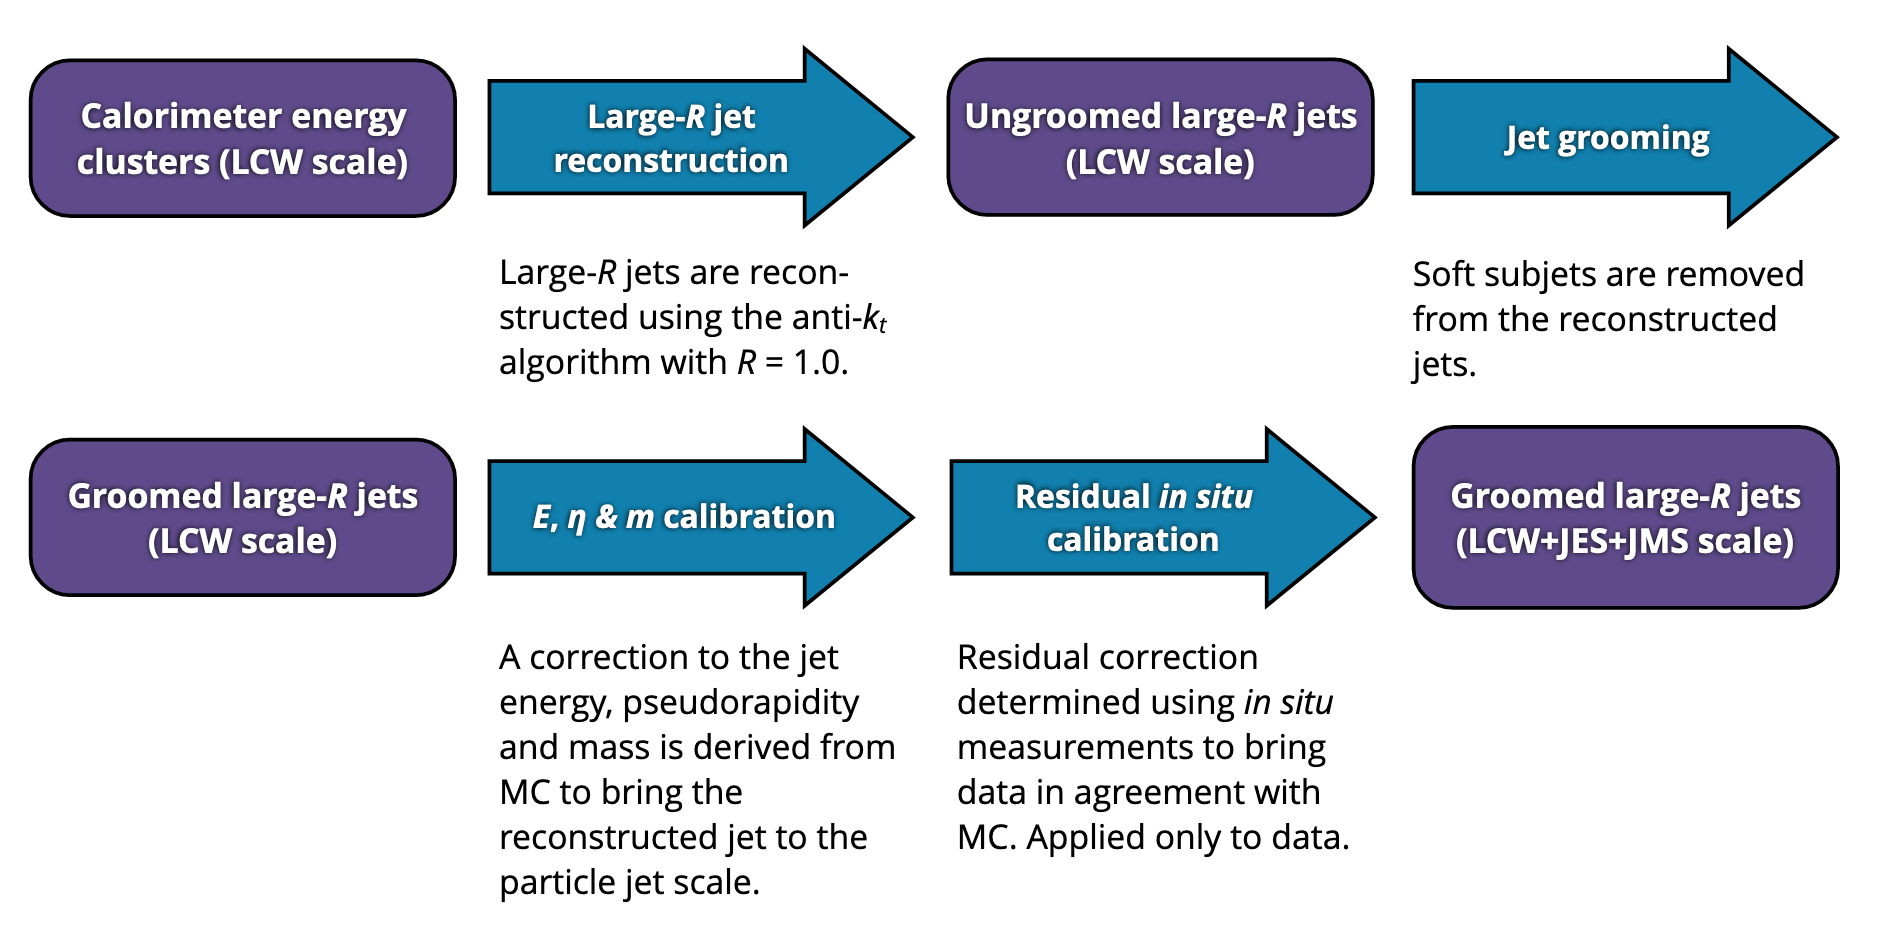
\includegraphics[width=\textwidth]{jet_calibration_flowchart}
	\caption{
	Overview of the large-$R$ jet reconstruction/calibration procedure, as described in \cite{Aaboud:2018kfi}.
	Note that for the TCC jets used in the analysis covered by this thesis, the inputs are Track-Calo Clusters (TCCs) instead of calorimeter clusters as specified in this chart.
	}
	\label{fig:jet_calib_flowchart}
\end{figure}

{
\newcommand{\EReco}{\ensuremath{E_{\mathrm{reco}}}}
\newcommand{\ETruth}{\ensuremath{E_{\mathrm{truth}}}}
\newcommand{\MReco}{\ensuremath{m_{\mathrm{reco}}}}
\newcommand{\MTruth}{\ensuremath{m_{\mathrm{truth}}}}
\newcommand{\CJES}{\ensuremath{c_{\mathrm{JES}}}}
\newcommand{\CJMS}{\ensuremath{c_{\mathrm{JMS}}}}
\newcommand{\EtaReco}{\ensuremath{\eta_{\mathrm{reco}}}}
Reconstructed jets are matched to particle-level jets with a simple angular matching procedure that minimizes their separation $\Delta R = \sqrt{(\Delta \phi)^2 + (\Delta \eta)^2}$.
The energy \textit{response} is defined as $\EReco / \ETruth$, where \EReco is the reconstructed jet energy \textit{prior} to calibration and \ETruth is the energy of the corresponding truth-level jet.
The mass response is defined similarly as $\MReco / \MTruth$.
The response is parameterized as a function of jet energy and $\eta_{\mathrm{reco}}$ and an average is computed ($R_E = \langle \EReco / \ETruth \rangle)$ using a Gaussian fit of the response. The jet energy response for TCC jets is shown in Figure~\ref{fig:tcc_jet_e_response}.

The energy correction derived this way (\CJES) is typically on the order of 5-10\% with only a weak dependence on the jet energy and a structure in $\eta_{\mathrm{reco}}$ that clearly reflects the detector technology and geometry.
The mass correction (\CJMS) is close to unity for jets with $p_T$ between 200 and 800 GeV, but can be as large as 1.5 for very energetic jets with low mass.

In addition to this jet energy scale (JES) and jet mass scale (JMS) calibration, a small correction $\Delta \eta$ is applied to correct for a bias relative to truth-level jets, but only in certain regions of the detector \cite{TheATLAScollaboration:2015soq}. 
At this point we refer to the uncalibrated quantities with subscript zero $(E_0, \eta_0$, etc), and the calibrated quantities with subscript ``reco''.
The final JES+JMS scale calibrated large-$R$ jet energy, mass, $\eta$ and $p_T$ can then be written as
\begin{align}
    \EReco &= \CJES\; E_0\\
    \MReco &= \CJES\; \CJMS\; m_0\\
    \EtaReco &= \eta_0 + \Delta \eta\\
    p_T^{\mathrm{reco}} &= \CJES \sqrt{E_0^2 - \CJMS^2 m_0^2}\; /\; \cosh{(\eta_0 + \Delta \eta)}
\end{align}
}

\begin{figure}
	\centering
	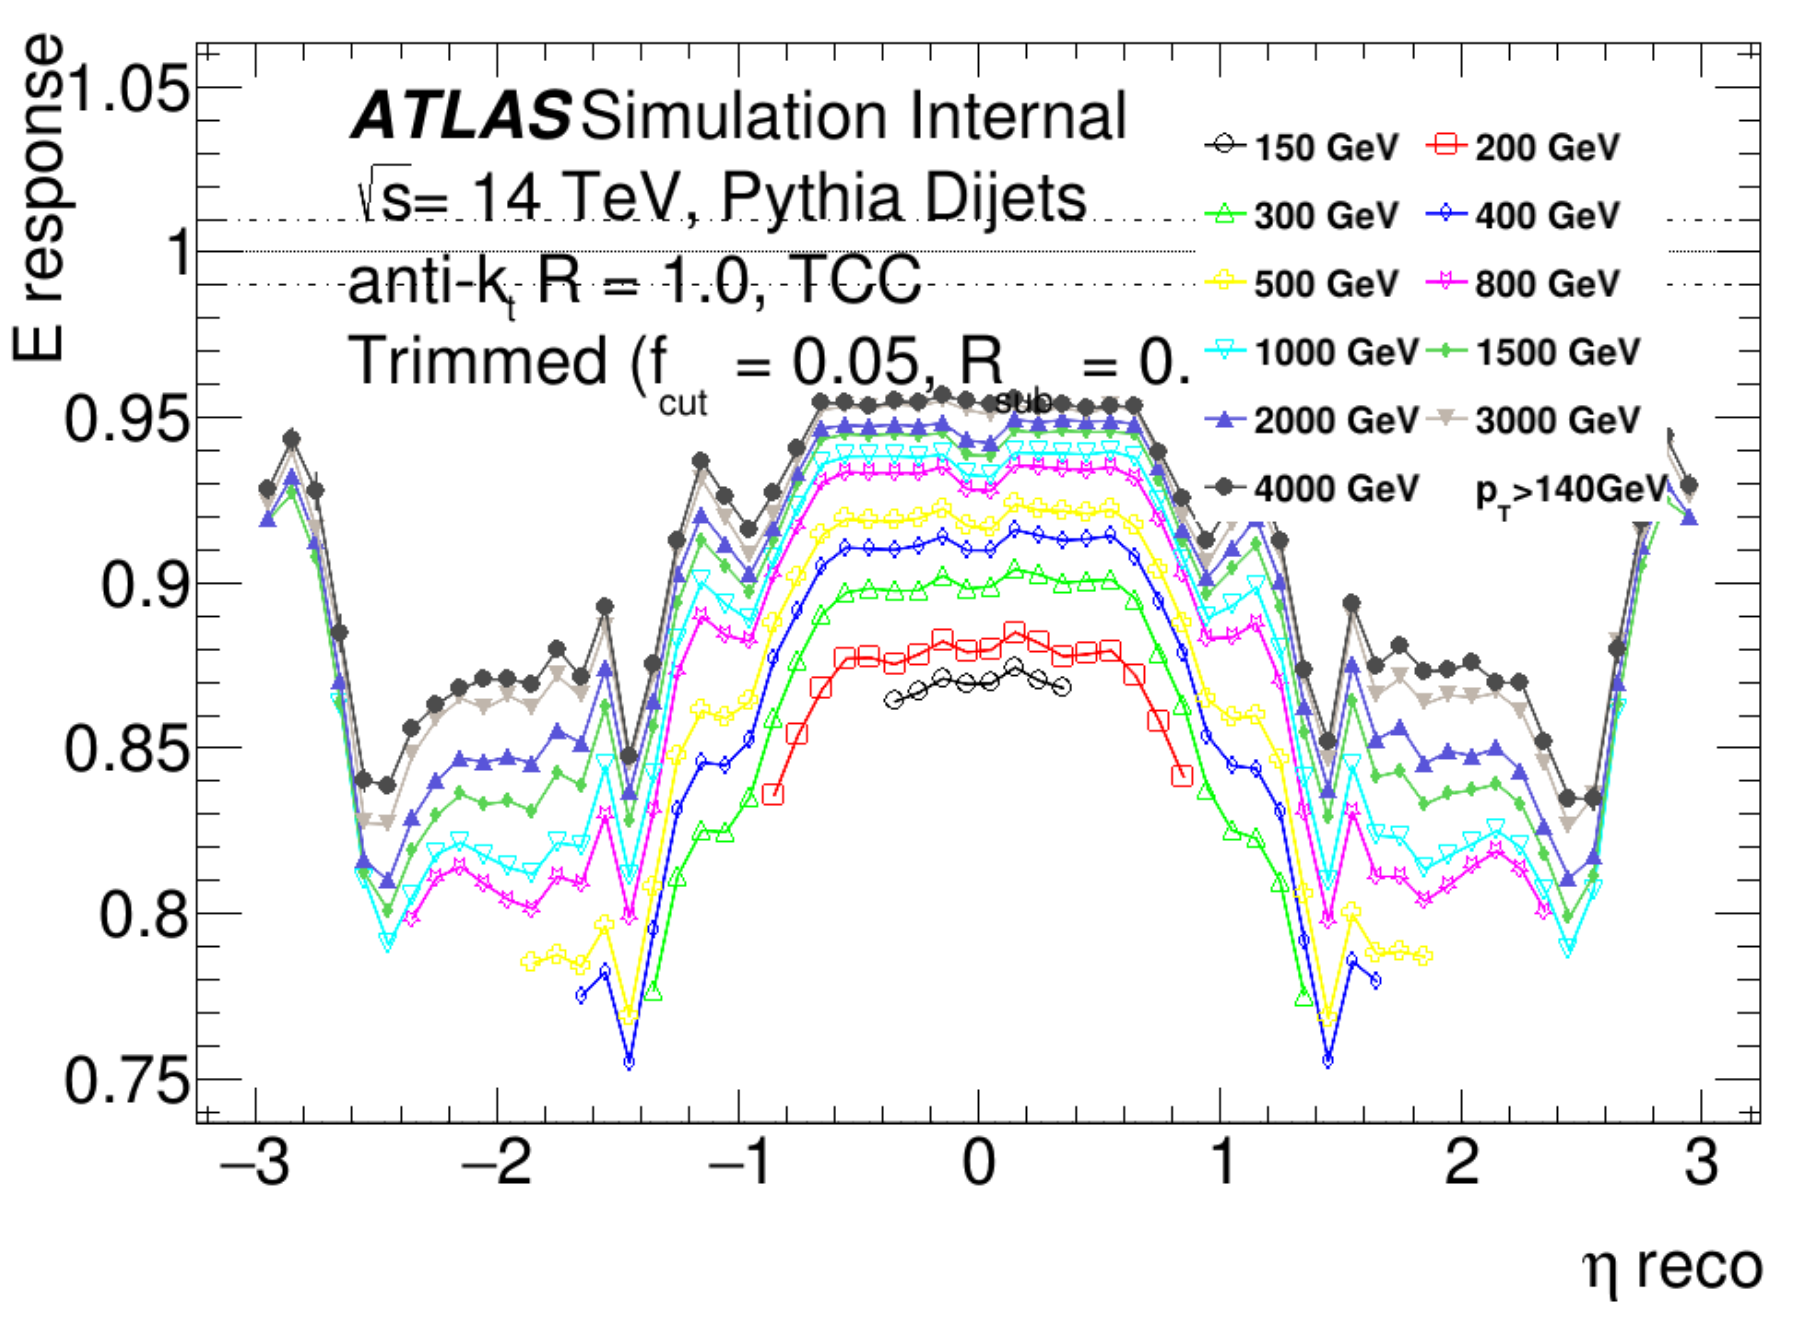
\includegraphics[width=0.6\textwidth]{tcc_jet_e_response}
	\caption{
	The jet energy response (before calibration) for TCC jets is presented as a function of jet pseodurapidity for several values of truth jet energy ranging from 150 GeV to 4 TeV.
	}
	\label{fig:tcc_jet_e_response}
\end{figure}

\section{Jet Substructure}
\label{sec:jet_substructure}
The primary goal of jet reconstruction is to accurately measure the four-vectors of the outgoing partons resulting from the hard scatter event.
However, a significant amount of additional information can be obtained by analyzing the internal structure of the jet constituents.
For example they may be diffuse and evenly spread out as will typically be the case in a gluon-initiated jet.
On the other hand, in the case of a $Z \rightarrow q\bar{q}$ or $H \rightarrow b\bar{b}$ decay there will be two distinct ``prongs'' corresponding to the separate decays of the quark pairs.
It is often the case that the sensitivity of jet-based searches can be improved by accounting for these differences in the internal structure of jets which differs for background and signal, because a single jet containing all the decay products of a massive particle (such as a $W$ or $Z$ boson) has significantly different internal structure than a jet (of the same $p_T$) originating from a light quark or gluon.

The details of jet substructure can be more clearly resolved if the contribution soft radiation and pileup is removed from the jet beforehand using a process generally referred to as \textit{jet grooming}.
For the lrage-$R$ TCC jets used for this thesis a technique called ``trimming'' is used which relies on the fact that the contamination from pile-up, multiple parton interactions (MPI) and initial state radiation (ISR) in the reconstructed jet is often much softer than the showering products of the partons associated with the outgoing hard-scatter.
During the trimming procedure soft constituents are removed by using their $p_T$ ratios as the metric for removal.

The trimming procedure uses a $k_T$ algorithm with a smaller radius parameter $R_{\mathrm{sub}}$ to reconstruct all constituents from a single large-$R$ jet into a set of smaller contained ``subjets''.
Any subjets with $p_{T_i} / p_T^{\mathrm{jet}} < f_{\mathrm{cut}}$ are removed from the original large-$R$ jet, where $p_{T_i}$ is the transverse momentum of the $i^{\mathrm{th}}$ subjet and $f_{\mathrm{cut}}$ is an adjustable parameter of the trimming procedure.
This process is illustrated in Figure~\ref{fig:jet_trimming_cartoon}.
For this thesis values of $R_{\mathrm{sub}} = 0.2$ and $f_{\mathrm{cut}} = 0.05$ are used.
A variety of alternative jet grooming procedures have been studied by ATLAS \cite{Aad:2013gja} as well, including methods that involve modifying the jet clustering algorithm itself.

\begin{figure}
	\centering
	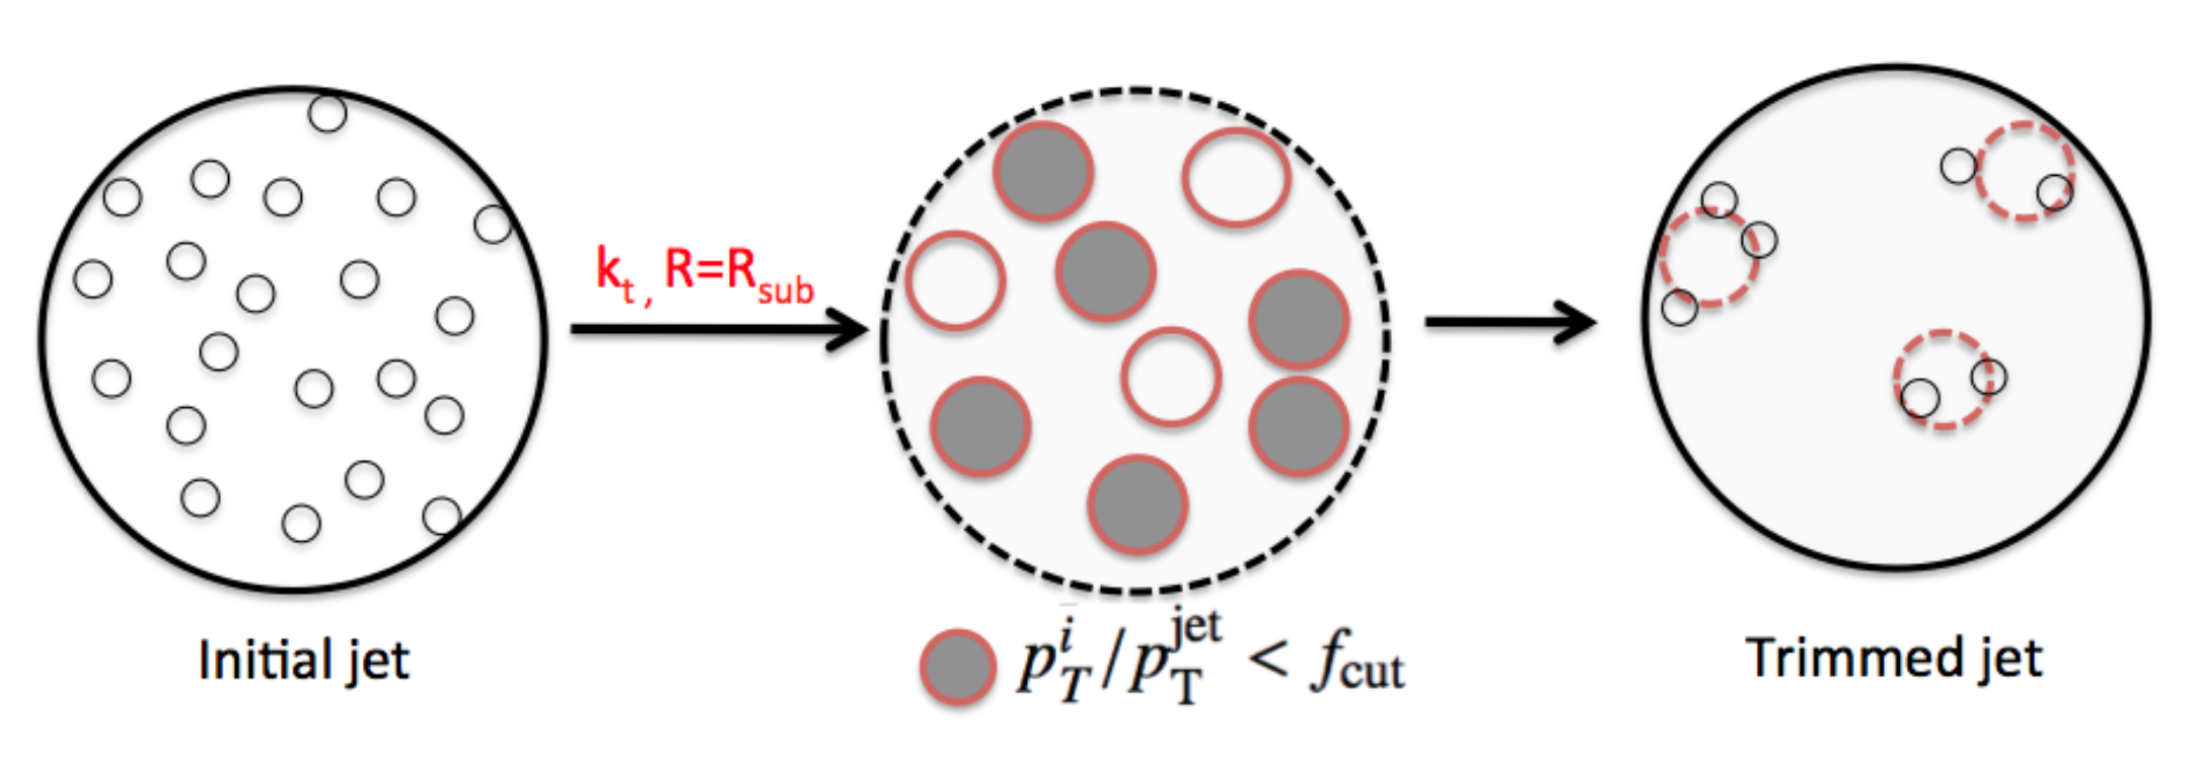
\includegraphics[width=0.6\textwidth]{jet_trimming_cartoon}
	\caption{
	Diagram depicting the jet trimming procedure.
    \cite{Aad:2013gja}
	}
	\label{fig:jet_trimming_cartoon}
\end{figure}

After jet grooming has been applied to enhance the quality of information contained within the constituents of a jet, the aggregate properties of these constituents can be computed with so-called \textit{jet substructure variables}.
In the past the more commonly used jet substructure variables were computed by analyzing the jet clustering algorithm history ($k_T$ ``splitting scales'' \cite{PhysRevD.65.096014}) or properties of the re-clustered subjets ($N$-subjettiness \cite{Thaler:2010tr}).

Presently, as is the case for the work covered in this thesis, the so-called \textit{Energy Correlation Functions} (ECF) \cite{Larkoski:2013eya, Moult:2016cvt} have become the de facto standard and are computed by summing certain expressions over all constituents contained within a jet as follows:
\begin{align}
    e_2^{(\beta)} &= \sum_{1 \le i < j \le n_J} z_i z_j \theta_{ij}^\beta \\
    e_3^{(\beta)} &= \sum_{1 \le i < j < k \le n_J} z_i z_j z_k \theta_{ij}^\beta \theta_{ik}^\beta \theta_{jk}^\beta \\
    e_4^{(\beta)} &= \sum_{1 \le i < j < k < l \le n_J} z_i z_j z_k z_l \theta_{ij}^\beta \theta_{ik}^\beta \theta_{jk}^\beta \theta_{il}^\beta \theta_{jl}^\beta \theta_{kl}^\beta
\end{align}
where $n_J$ is the number of particles in the jet, $\beta$ is an adjustable parameter, $z_i$ is the ratio of the $p_T$ of the $i^{\mathrm{th}}$ constituent of the jet over the total jet $p_T$, and $\theta_{ij} = (\phi_i - \phi_j)^2 + (y_i - y_j)^2$ is the angular separation of constituents $i$ and $j$.
These ECF expressions form the basis for constructing higher-level jet substructure observables where $e_{N+1}^{(\beta)}$ captures the $N$-prong nature of a jet. For example, the high level jet substructure observable that quantities how compatable a jet is with a 2-prong structure is
\begin{equation}
    D_2^{(\beta)} = \frac{e_3^{(\beta)}}{\left( e_2^{(\beta)} \right)^3} \end{equation}
The $e_2$ vs. $e_3$ phase space distribution of 1-prong (light quark/gluon) and 2-prong ($W/Z \rightarrow q\bar{q}^{(\prime)},\ H \rightarrow b\bar{b})$ jets are shown in Figure~\ref{fig:d2_plane_contours}.
The value $\beta = 1$ is standard in ATLAS as it results in the highest sensitivity across a wide range of jet mass and $p_T$.

\begin{figure}
	\centering
	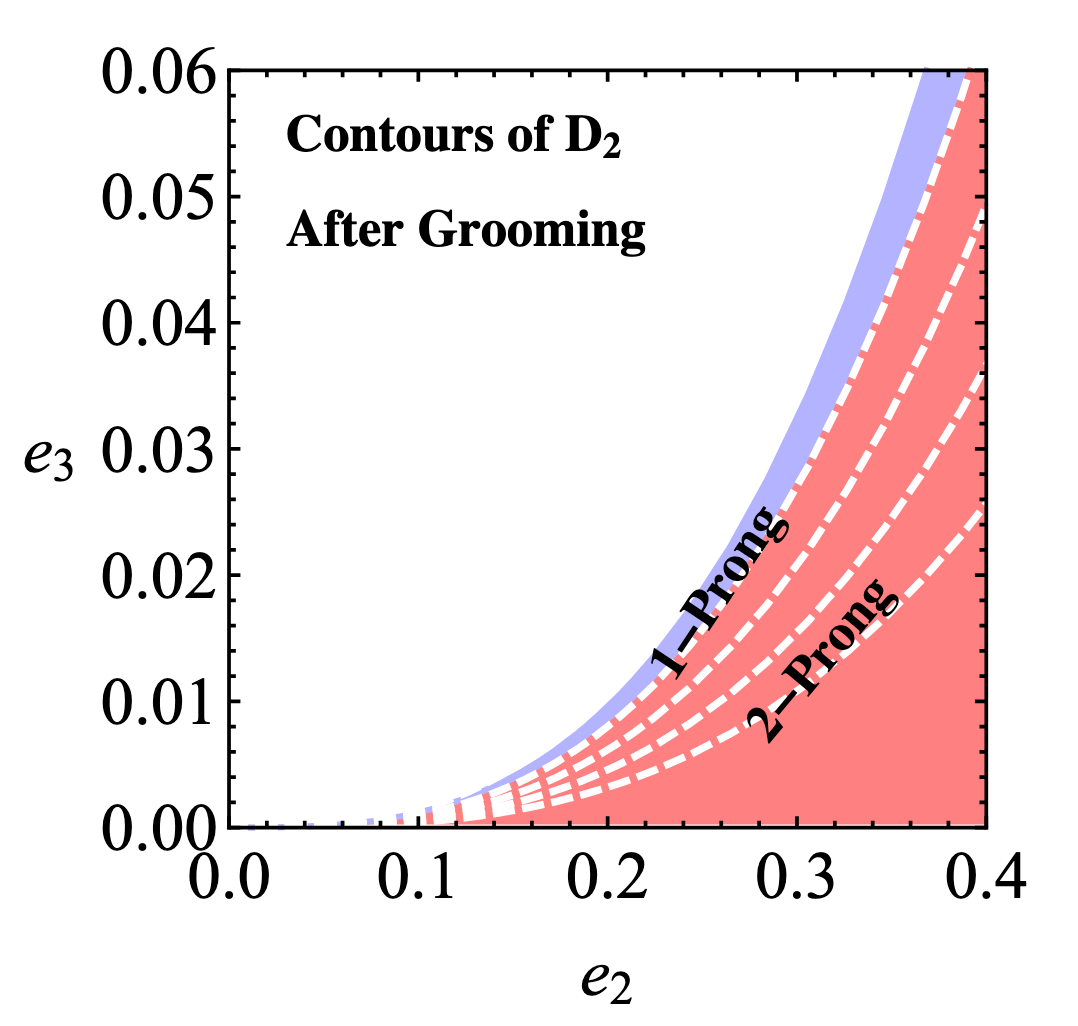
\includegraphics[width=0.6\textwidth]{d2_plane_contours}
	\caption{
	Schematic depiction of the phase space for the energy correlation functions $e_2$ and $e_3$ which compose $D_2$.
	Contours of the $D_2$ variable are shown as white dashed curves.
	The $D_2$ variable is explicitly defined to cleanly separate the 1-prong and 2-prong regions of this phase space.
    \cite{Moult:2016cvt}
	}
	\label{fig:d2_plane_contours}
\end{figure}

\section{B-Jet Identification}
\label{sec:btagging}
In general jet reconstruction algorithms proceed without special consideration of the ``flavor'' of a jet: light quark, charm ($c$) or bottom ($b$).
However, the identification of jets containing $b$-hadrons (often simply called $b$-\textit{jets}) is of utmost importance not only for this thesis, but for the majority of the most ambitious physics goals of the ATLAS experiment.
In particular the precision measurements of Higgs boson properties and searches for BSM physics rely heavily on an ability to pick out or \textit{tag} $b$-jets and distinguish them from light quark jets. The algorithms used to perform this tagging are referred to as \textit{b-tagging algorithms}.

The relatively long lifetime of $b$-hadrons (approximately 1.5 picoseconds) gives them a characteristic flight path of approximately 5 mm from the primary hard-scatter vertex before undergoing secondary decay.
This flight distance is quite often large enough that the decay chain can be resolved by the ID and the secondary decay vertex (SV) can be identified.
Furthermore, roughly 90\% of the time a tertiary vertex (TV) from a $c$-quark will be present as well.
These properties, depicted in Figure~\ref{fig:b_decay_cartoon}, are exploited by the $b$-tagging algorithms.

\begin{figure}
	\centering
	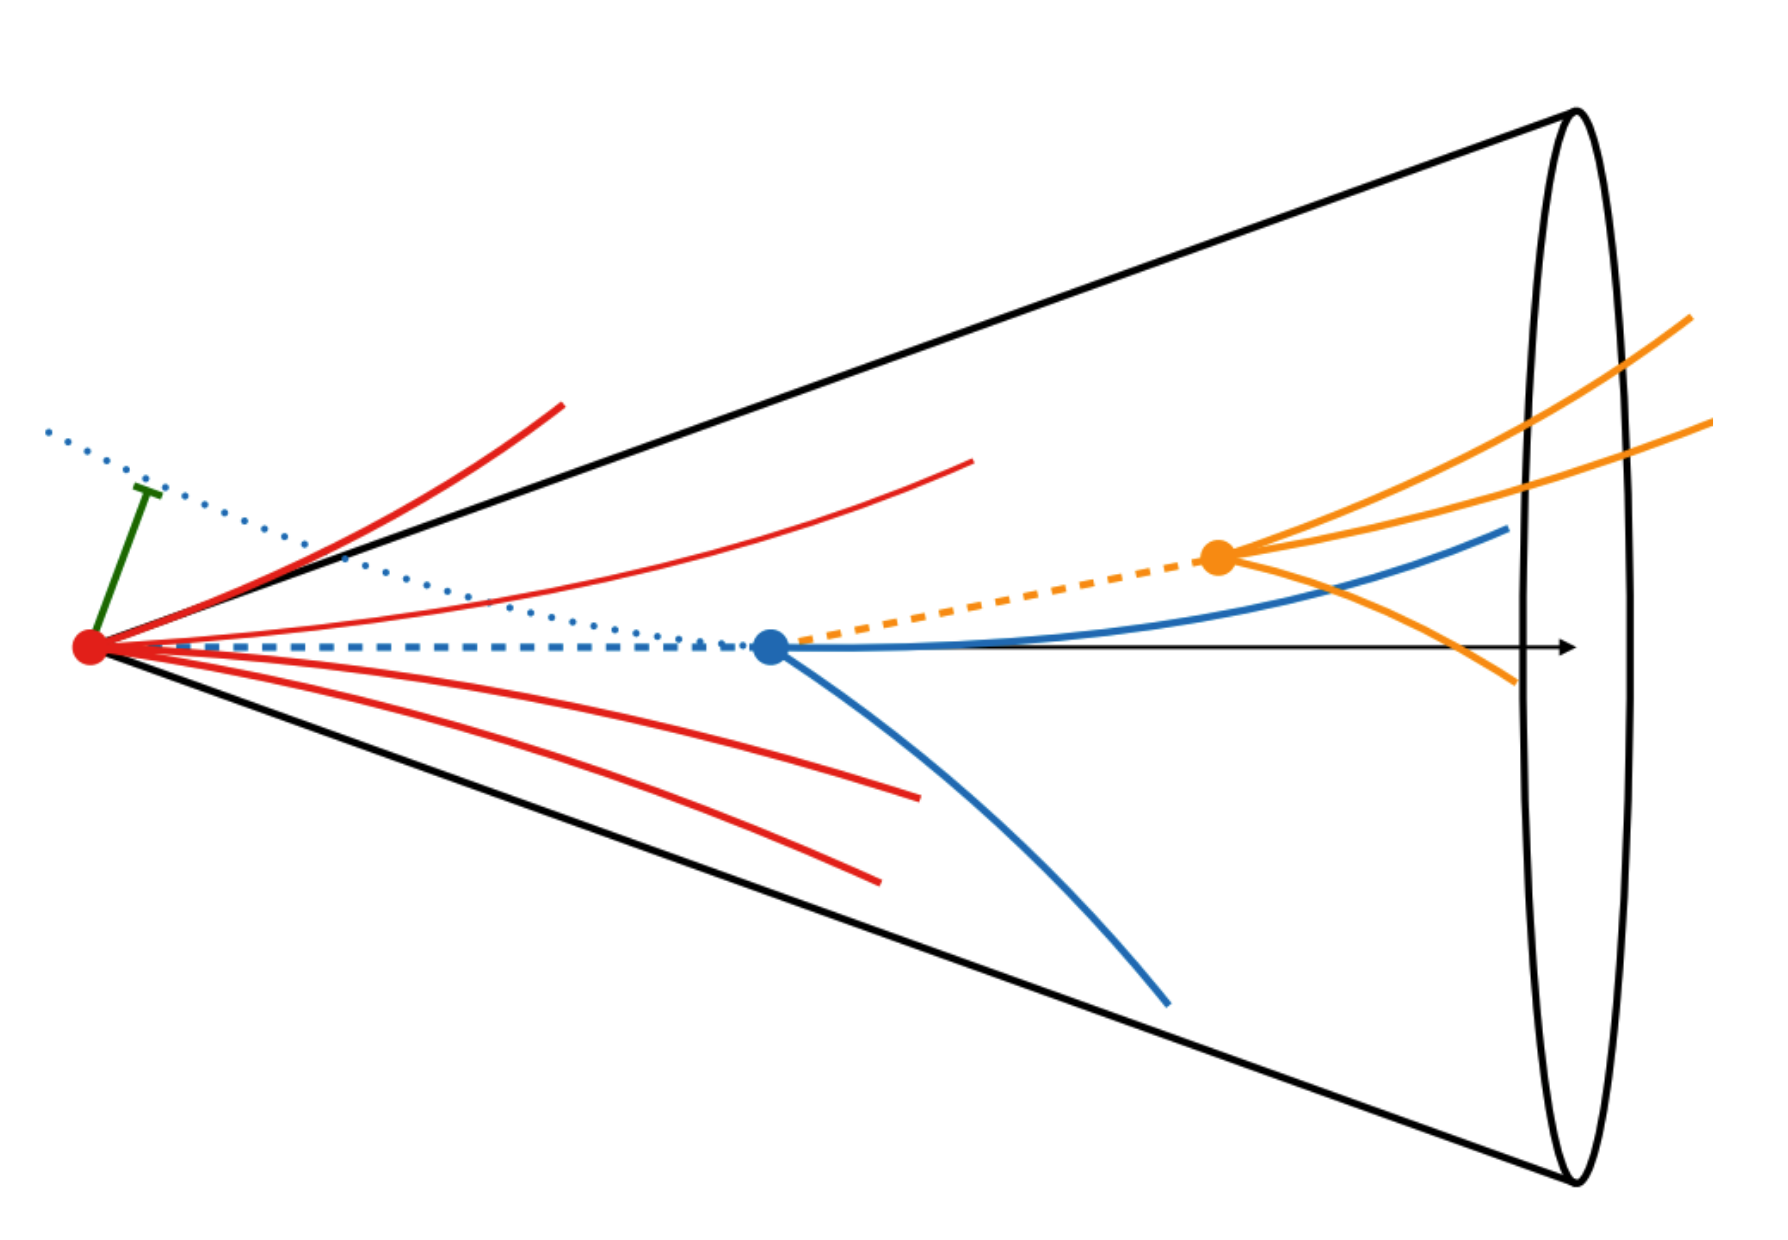
\includegraphics[width=0.65\textwidth]{b_decay_cartoon}
	\caption{
	Cartoon of a $b$-jet decay containing a $b$-hadron decay vertex (blue dot) displaced from the primary $pp$ vertex (red dot) and a $c$-hadron vertex (orange dot) further displaced and often close to the $b$-hadron flight axis.
	The secondary (blue dot) and tertiary (orange dot) vertices have large impact parameters (green line) with respect to the primary hard scatter vertex (red dot). \textcopyright 2017 Andy Chisholm.
	}
	\label{fig:b_decay_cartoon}
\end{figure}

The primary $b$-tagging algorithm developed for ATLAS during Run 2, referred to as MV2c10, utilizes a machine learning technique called a boosted decision tree (BDT).
This is multivariate algorithm which uses inputs from a variety of other algorithms which utilize both tracking and calorimeter information pertintant to each jet under consideration. These include:
\begin{itemize}
    \itemsep0em 
    \item Jet $p_T$ and $\eta$.
    \item A likelihood-based combination of the transverse and longitudinal impact parameter significances. %TODO: cite relevant thesis section
    \item The presence and properties of a secondary vertex.
    \item Reconstruction of a $b$-hadron decay chain using a Kalman filter to search for a common direction connecting the primary vertex to both the bottom and tertiary charm decay vertices.
\end{itemize}

The MV2c10 machine learning algorithm is trained on a set of events from a simulated $t\bar{t}$ sample, where $b$-jets are labelled as ``signal'' and $c$-jets and light quark jets are labelled as ``background''.
Ultimately the MV2c10 produces a single output discriminating variable for each jet, as shown in Figure~\ref{fig:mv2c10_discriminant}.

\begin{figure}
	\centering
	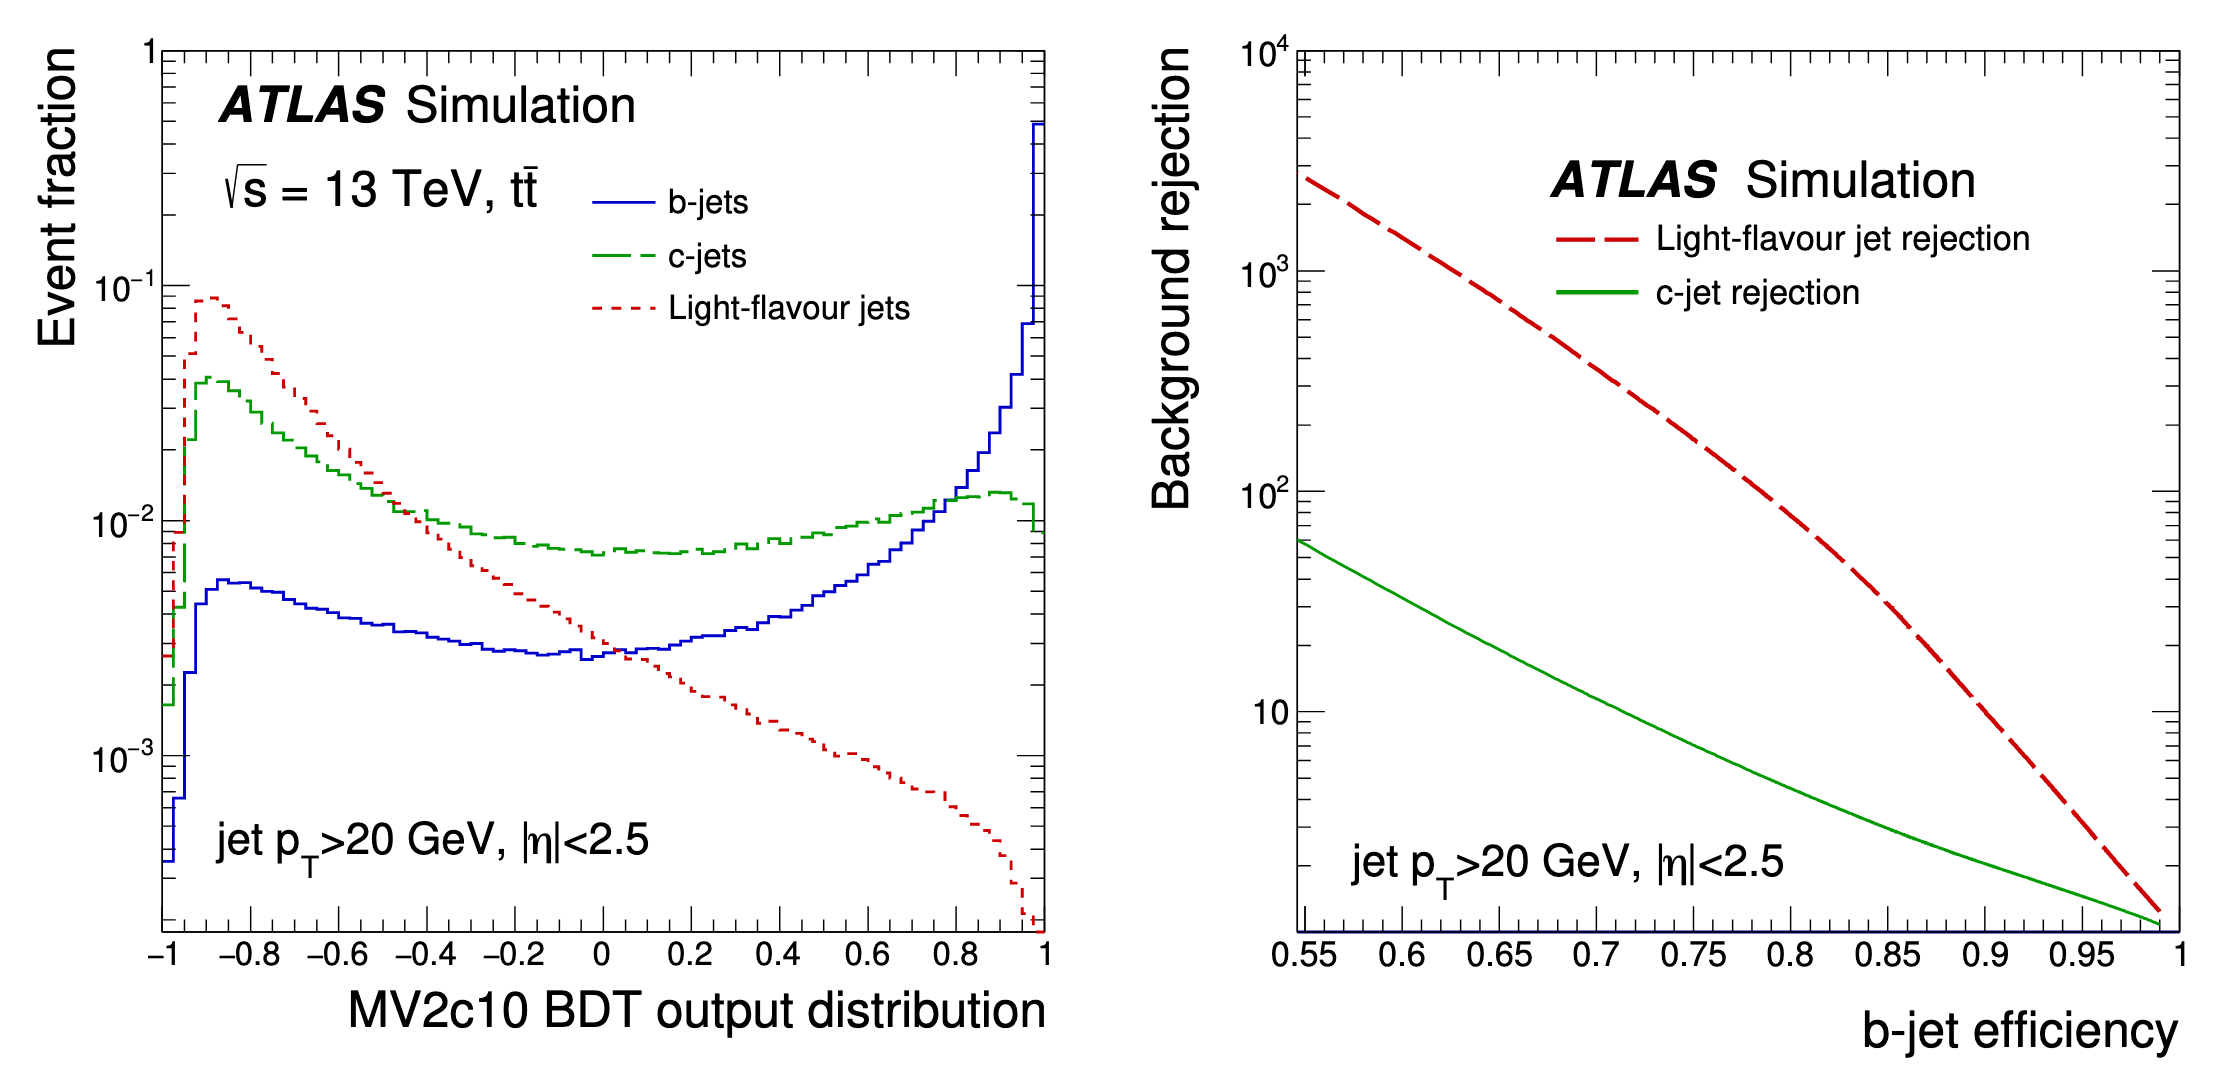
\includegraphics[width=\textwidth]{mv2c10_discriminant}
	\caption{
	The MV2c10 output (left plot) for $b$-jets (solid line), $c$-jets (dashed lined) and light quark jets (dotted line) in simulated $t\bar{t}$ events, as well as the background rejection for light quarks (dashed line) and $c$-jets as a function of the $b$-jet tagging efficiency (right plot).
	This performance was evaluated on simulated $t\bar{t}$ events.
    \cite{Aaboud:2018xwy}
	}
	\label{fig:mv2c10_discriminant}
\end{figure}

In order to utilize the MV2c10 output discriminant in a physics analysis, two tasks must be accomplished: (1) Cuts on the MV2c10 discriminant called ``working points'' (WP) must be defined, with a specified signal efficiency in simulated events and (2) scale factors to correct for small discrepancies between simulation and data must be derived along with their uncertainties.
The ATLAS experiment produces these scale factors by studying a very pure $t\bar{t}$ sample in data using two complementary methods: a ``tag-and-probe'' approach (T\&P) and a combinatorial likelihood approach (LH).
These methods both rely on the fact that the $t \rightarrow Wb$ branching fraction is close to 100\%.
Two oppositely charged leptons resulting from the leptonic $W$ boson decays are required in each event ($e\mu$, $ee$ or $\mu\mu$).
By selecting only events where both $W$ bosons (from each top quark) decay leptonically, the number of non $b$-jets in these events is greatly reduced. The T\&P and LH methods differ in the restrictions they place on the lepton flavors of the final state. The resulting $b$-tagging efficiencies and scale factors are shown in Figure~\ref{fig:b_tagging_eff_sf} for the 70\% WP.

\begin{figure}
	\centering
	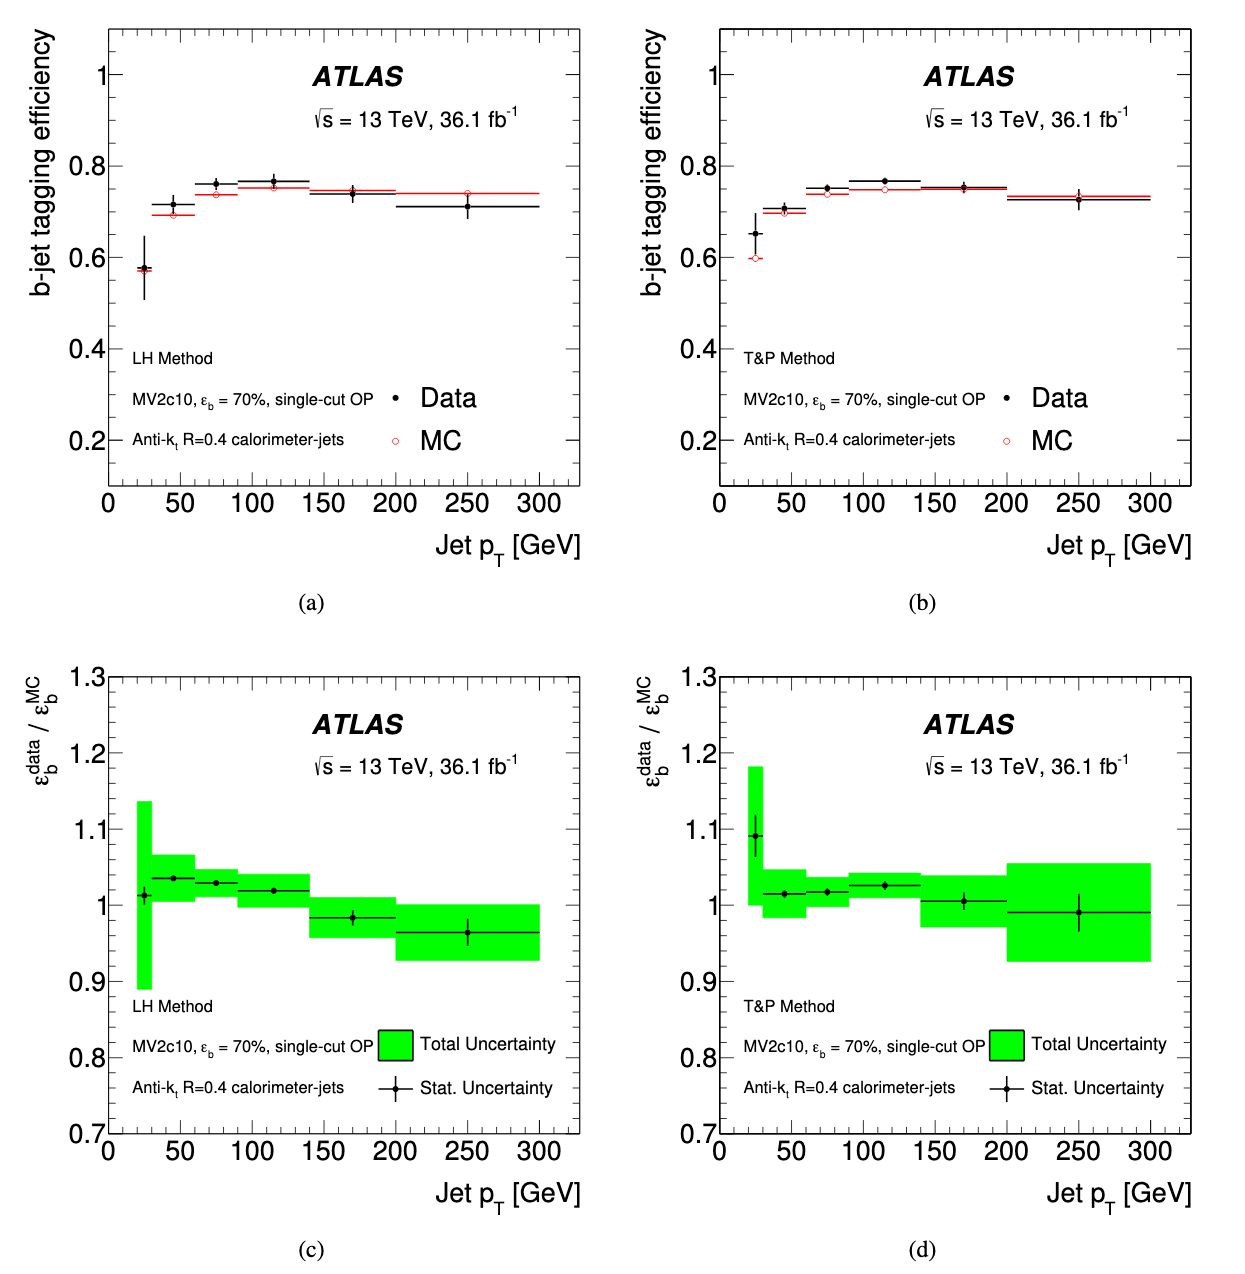
\includegraphics[width=\textwidth]{b_tagging_eff_sf}
	\caption{
	Top: The $b$-jet tagging efficiency measured in data (full circles) and simulation (open circles), corres-ponding to the 70\% $b$-jet tagging efficiency single-cut OP, as a function of the jet $p_T$ using (a) the LH method and (b) the T\&P method, for $R = 0.4$ calorimeter-jets. The error bars correspond to the total statistical and systematic uncertainties. Bottom: Data-to-simulation scale factors as a function of the jet $p_T$ using (c) the LH method and (d) the T\&P method. Both the statistical uncertainties (error bars) and total uncertainties (shaded region) are shown.
    \cite{Aaboud:2018xwy}
	}
	\label{fig:b_tagging_eff_sf}
\end{figure}

